\documentclass{beamer}
 
\usepackage[utf8]{inputenc}
\usepackage{amsmath}
\usepackage{amssymb}
\renewcommand\mathfamilydefault{\rmdefault}

 
 
%Information to be included in the title page:
\title{Combinatorics: Introduction}
\author{Ben Kettle}
\date{10 Jan 2020}
 
\begin{document}
 
\frame{\titlepage}
 
\begin{frame}{Warm-Up Exercises}
\begin{enumerate}
    
    \item A certain website requires passwords of two letters, followed by 8 digits. For example, AB12345678 would be a valid password. If no repeated characters are allowed, how many possible passwords exist?
    
    \item Instead, if no consecutive repetition is allowed, how many password options are there? For example, AA12345678 is not allowed but AB121345678 is.
    
    \item Suppose we have a grid with 9 rows and 3 columns. Each square can be colored either black or white. Is it possible for every row to be different from every other?
    
\end{enumerate}
\end{frame}

\begin{frame}{Permutations}
    The first example problem brings us to \alert{permutations}, or arrangements of the items in a set. 
    
    \begin{itemize}
        \item How many permutations exist of the items in the set $\{a, b, c\}$?
    \end{itemize}
    
    \visible<2->{Again, for clarity, we can solve this using a tree, dividing the ordering into a "slot" for each place. 
    
    \begin{figure}
        \centering
        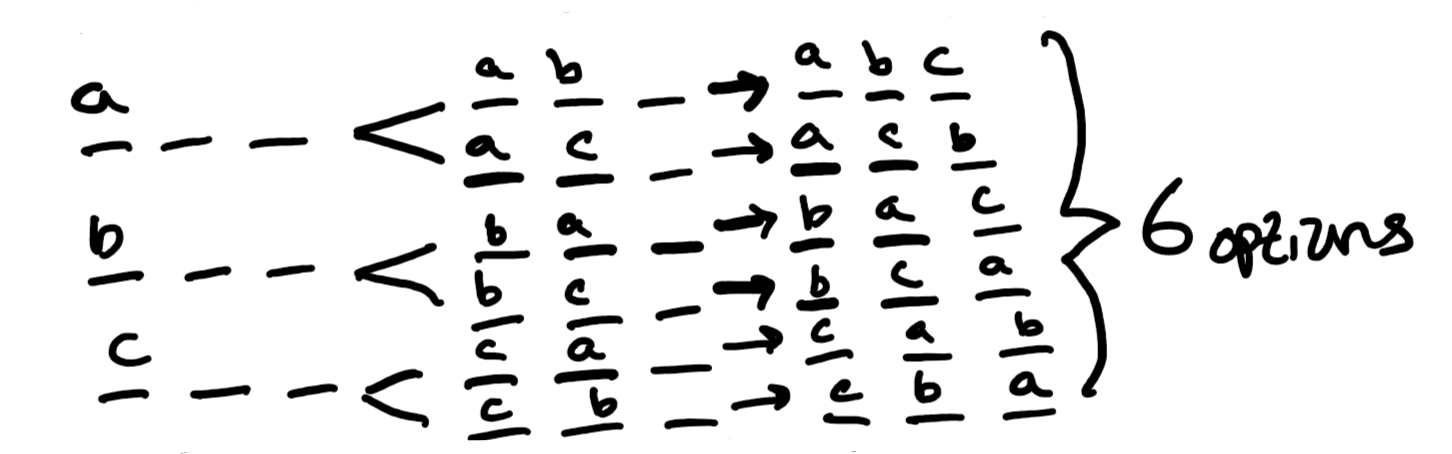
\includegraphics[scale=.3]{permtree.png}
    \end{figure}
    
    First, we consider all the options for the first "slot" (3) Then, we consider the number of options for the second slot in each of these cases (2). Finally, we fill in the 3rd spot with its (1) option for each case so far. This leaves us with 6 options clearly.}
\end{frame}

\begin{frame}{Permutations Formally}
    Permutations are pretty uninteresting at first glance, but are used over and over again throughout combinatorics. So once again, we want an easy way to calculate how many permutations of a set exist.
    
    \visible<2->{Following the same steps as in the tree, we can see that for an $n$-element set, there are $n$ options for the first slot $n-1$ for the 2nd, and so on, until $1$ option for the final slot. Applying the product rule to find the size of all permutations:
    
    \[ n(n-1)(n-2)\cdots2\cdot1 \]
    
    This is simply equal to $n!$. So for any $n$-element set, there are $n!$ permutations of that set. 
    }
\end{frame}

\begin{frame}{Permutation Exercises}
    \begin{itemize}
        \item How many permutations are there of the set $\{a, b, c, d, e, f, g, h\}$?
    \end{itemize}
\end{frame}

\begin{frame}{Division Rule}
    Before we do an example with permutations, we must explain the division rule, another key concept for many combinatorics problems. For example, if we assume all cars have 4 wheels, counting all the wheels in a parking lot and finding the number of cars inside the garage, this would be an application of the division rule. \vspace{5mm}
    
    \textbf{Definition:} Division Rule \newline
    If $f: A \rightarrow B$ is $k$-to-$1$, then $|A| = k\cdot |B|$.
\end{frame}

\begin{frame}{Exercise}
    \begin{itemize}
        \item How many unique ways can we arrange the letters in the word PRIOR? 
    \end{itemize}
\end{frame}

\begin{frame}{Round Table Example}
    Imagine the small group of students you are with is sitting around a round table. We want to find all the different arrangements of students, where "different" means that one arrangement cannot be simply a rotation of another. For example, these are considered equal arrangements:
    \begin{center}
        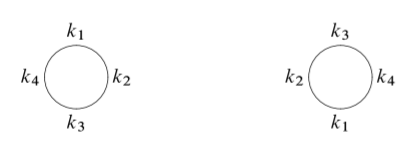
\includegraphics[scale=.7]{roundequiv.png}
    \end{center}
    How can we think about this problem in terms of sets and permutations?
\end{frame}

\begin{frame}{Creating a Mapping}
    We can create a mapping from each ordering $(k_i, k_j, k_l, k_m)$ to a table arrangement by starting at the top and assigning seats counterclockwise:
    
    \begin{center}
    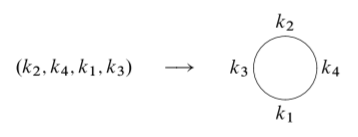
\includegraphics[scale=.7]{roundex1.png}
    \end{center}
    
    But this isn't all---the ordering $(k_3, k_2, k_4, k_1)$ should be counted as the same arrangement. Which other sequences map to this orientation? How many are there? What kind of mapping exists?
    \visible<2->{
    \begin{center}
        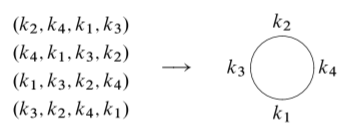
\includegraphics[scale=.7]{roundex2.png}
    \end{center}}
\end{frame}

\begin{frame}{Applying the Division Rule}
    We can see that there is a 4-to-1 mapping in this case, so each arrangement has 4 corresponding permutations. How can we use this to find the total number of arrangements?\vspace{5mm}
    
    \visible<2->{Because this is a 4-to-1 mapping between orderings $O$ and arrangements $A$, the division rule tells us that $|A| = \tfrac{|O|}{4}$. We can then solve for the size of the set of arrangements easily.}
\end{frame}

\begin{frame}{Permutations of a Certain Size}
    It's also very useful to find all the orderings of $k$ elements from an $n$ element set. For example, if the bookshelf in your house has 10 books, and you have a lazy weekend day and want to read 3 of them, we can use this to calculate all the different ways you can spend your day. \vspace{2mm}
    
    Does anyone know how we might find this value? \visible<2->{\alert{It's good to think about this problem as another use of the division rule. Here, we once again want to find permutations, but only care about the \textit{first three items}. Any set of permutations where the first three items are the same should all count as only one book arrangement. For example, if our books are labelled A-J:
    
    \[ \left. \begin{array}{c}
         ABCDEFGHIJ \\
         ABCJIHGFED \\
         ABCDJIEHFG \\
         \vdots
    \end{array} \right\} ABC\textbf{XXXXXXX} \]}}
\end{frame}

\begin{frame}{Permutations of a Certain Size: Creating a Mapping}
    Because we only care about these first three slots, we can once again create a mapping from permutations to book selections. Continuing with the example, we need to find how many permutations of the 10 books correspond to each 3-book ordering. 
    
    \[ \left. \begin{array}{c}
         \textbf{ABC}DEFGHIJ \\
         \textbf{ABC}JIHGFED \\
         \textbf{ABC}DJIEHFG \\
         \vdots
    \end{array} \right\} \textbf{ABC}XXXXXXX \]
    
    \visible<2->{Notice that for each ordering of the first three books, the remaining 7 slots can be any permutation of the remaining 7 books. 
    \begin{itemize}
        \item Given what we know about permutations, how many permutations on the left correspond to each item on the right? \visible<3->{Because anu permutation of the 7 books fits, there are 7! options for each 3-book ordering.}
    \end{itemize}}
    
\end{frame}

\begin{frame}{Applying the Division Rule}
    Continuing with the example from the last side, we can then apply the division rule.
    \begin{itemize}
        \item How many different 3-book orderings are there from a shelf of 10 books? \visible<2->{\alert{The division rule tells us that for the set of permutations $P$ and orderings $O$, $|O|=\frac{|P|}{7!}$ orderings. We know there are $10!$ orderings of 10 elements, so $|O|=\frac{10!}{7!}$.}}
    \end{itemize}
    
    \visible<3->{We want to generalize this to find the number of orderings of $k$ elements from an $n$-element set. Does anyone have an idea of how to do this? 
    \vspace{2mm} 
    
    \visible<4->{We will always have a similar format where we only care about the first $k$ elements, so we can write this as:
    
    \[ \frac{n!}{(n-k)!} \]}}
\end{frame}

\begin{frame}{When Order Doesn't Matter}
    What if we don't care about order? For example, say we want to choose 2 fruits for a smoothie from a set of 5 options. Does anyone have an idea of how we can get from what we had in the last slide to what we have now? \vspace{2mm}
    
    \visible<2->{What we found in the last slide gives us every permutation of 2 fruits where order \textit{does matter}. But that number would count $\{apple, banana\}$ and $\{banana, apple\}$ separately. So once again, we need to apply the division rule to eliminate this \alert{over-counting}. 
    \begin{itemize}
        \item What do we need to divide by in order to eliminate this over-counting? \visible<3->{In this case, we want to convert our permutations of 2 elements into simply sets of 2 elements. We know that for a set of 2 elements, there are $2!$ corresponding permutations, so we can divide by $2!=2$.}
    \end{itemize}}
\end{frame}

\begin{frame}{Combinations}
    Once again, we want to find a way to generalize this into \alert{combinations} of $k$ elements from an $n-element$ set. Remember that we first find $k$ element \textit{orderings}, and then further reduce those orderings to eliminate sequences with the same elements but different orderings. Can someone combine the last few parts to find a formula for $k$-element combinations of an $n$-element set?
    
    \visible<2->{Because there are $k!$ ways to arrange the items in a subset of $k$ items, there exists a $k!$-to-$1$ mapping from permutations of size $k$ (calculated previously) to subsets of size $k$. Thus, we can use the division rule and divide out $k!$ to find the formula we are looking for.}
\end{frame}

\begin{frame}{Combinations and Binomial Coefficient}

    \textbf{Definition:} Combinations \newline
    A combination is a selection of items in which the order does not matter. For a set of $n$ elements, the size of the set of all $k$-element combinations is given by:
    
    \[ \binom{n}{k} = \frac{n!}{k!(n-k)!} \]
    
    When reading this aloud, you can refer to this number as "n choose k". Because we use combinations so often, we also define this notation called the \alert{binomial coefficient}, which is what you see on the right side.
\end{frame}

\begin{frame}{Exercises}
    \begin{itemize}
        \item How many binary sequences of length 8 contain exactly 2 ones? \textit{hint: think about how we calculated the number of subsets last week}
    \end{itemize}
\end{frame}

\end{document}
